 % =====================================================================
%  Conference poster
%  "Enhancing Angular Sensitivity of Segmented Antineutrino Detectors
%   for Reactor Monitoring"
%
%  Target: Neutrino 2026, 4 ft x 3 ft landscape
%          (48" x 36" = 121.92 cm x 91.44 cm)
%  A0 fallback: comment-swap the \usepackage[...]{beamerposter} line.
% =====================================================================
%%% To-Do %%%
% [ ] Finalize Affiliate Seals
% [X] Fix references to non-placeholder set
% [X] Update figure caption reference rendering bug (currently rendering as [?])
% [ ] Update figures to have consistent formatting and coloring
% [X] Add section content for Block 1
% ----> [ ] Finalize text content
% ----> [ ] Finalize object placement
% ----> [X] Update figure captions to fit poster context
% [X] Add section content for Block 2
% ----> [ ] Finalize text content
% ----> [ ] Finalize object placement
% ----> [ ] Update figure captions to fit poster context
% [X] Add section content for Block 3
% ----> [ ] Finalize text content
% ----> [ ] Finalize object placement
% ----> [ ] Update figure captions to fit poster context
% [X] Add section content for Block 4
% ----> [ ] Finalize text content
% ----> [ ] Finalize object placement
% ----> [ ] Update figure captions to fit poster context
% [X] Draft results section content for Block 5
% ----> [ ] Finalize text content
% ----> [ ] Finalize object placement
% ----> [ ] Update figure captions to fit poster context
% [X] Update contributors list
% [X] Update Acknowledgements section
% [X] Add QR code to Paper B
% [X] Fix horizontal text clipping issue in body blocks
% [X] Adjust Acknowledgements section to fix text clipping (move left margin to left while keeping right margin inplace)

%%% Notes 5/31/26
% 1. Updated poster dimensions from A0 -> 4'x3'. 
% 2. Set minimum font size template-wide to render at 28pt with the exception of in-figure text and superscripts for references.
% 3. Updated the rendering for the "To-Scale" diagram in Block 1 to actually be to-scale when the poster is rendered at 100%. It's much smaller and the in-figure text will not be 28 pt.
% 4. Printed out the 100% scale poster as a grid of 25 pages and arranged them to check how each of the assets would look. So far everything is looking really good and the text is easily readable at poster scale.
% 5. Fixed the margins for each of the body columns and for the internal text rendering.
% 6. Increased scaling for Figure 6 and moved overlapping labels to right side to served as a plot legend instead.

%%% Notes 5/15/26 %%%
% Logos are still in draft stage
% Contributor list still placeholder names
% Reference list still placeholder
% Acknowledgements list still placeholder
% Rough outline w/draft-version figures @ https://docs.google.com/presentation/d/1dbpYslNvso42dSGUwl4KMoec9q9DDa_qAD9pkKTYXmQ/edit?slide=id.p#slide=id.p
% QR code to Paper B arxiv link generated and in project repo
% Figures currently not in colorblind-friendly format



\documentclass[final]{beamer}
\usepackage[size=custom,width=121.92,height=91.44,scale=1.25]{beamerposter}
% A0 fallback (swap the line above for this one):
% \usepackage[size=a0,orientation=landscape,scale=1.25]{beamerposter}

% ---- packages -------------------------------------------------------
\usepackage[T1]{fontenc}
\usepackage[utf8]{inputenc}
\usepackage{lmodern}
\usepackage{helvet}
\renewcommand{\familydefault}{\sfdefault}
\usepackage{graphicx}
\usepackage[percent]{overpic}
\usepackage{pict2e}
\usepackage{epsfig}
\usepackage{tikz}
\usetikzlibrary{positioning,arrows.meta,calc,backgrounds,
                shapes.geometric,decorations.pathreplacing,fit}
\usepackage{xcolor}
\usepackage{amsmath,amssymb,bm}

\let\OldDelta\Delta
\renewcommand{\Delta}{\mathnormal{\OldDelta}}
\usepackage{siunitx}
\usepackage{enumitem}
\usepackage{caption}
\usepackage{microtype}
\usepackage{booktabs}
\usepackage[framemethod=tikz]{mdframed}

% ---- palette --------------------------------------------------------
\definecolor{UHGreen}{HTML}{024731}
\definecolor{UHGold}{HTML}{C8A464}
\definecolor{LLNLNavy}{HTML}{003594}
%\definecolor{BlockBG}{HTML}{F5F4EE}
\definecolor{BlockBG}{HTML}{FFFFFF}

\definecolor{SoftGrey}{HTML}{ECECEC}

% ---- beamer theme ---------------------------------------------------
\setbeamercolor{block title}{fg=white,bg=UHGreen}
\setbeamercolor{block body}{fg=black,bg=BlockBG}
\setbeamerfont{block title}{size=\Large,series=\bfseries}
\setbeamerfont{block body}{size=\normalsize}
\setbeamertemplate{itemize item}%
  {\color{UHGreen}\raisebox{0.05ex}{\textbf{\textbullet}}}
\setbeamertemplate{itemize subitem}%
  {\color{UHGreen}\raisebox{0.1ex}{\textendash}}
\setbeamertemplate{navigation symbols}{}
\setbeamertemplate{caption}[numbered]{}
\setbeamertemplate{caption label separator}{:~}
\setbeamerfont{caption}{size=\small}

\newlength{\ribbonheight}
\setlength{\ribbonheight}{2.5cm}
\newlength{\blockpadding}
\setlength{\blockpadding}{0.8cm}% internal L/R padding = P (mirrors \blockinnerpad)
\setbeamertemplate{block begin}{%
  \vspace*{-0.3ex}%
  \begin{beamercolorbox}[wd=\linewidth,sep=0pt,leftskip=0pt,rightskip=0pt,colsep*=0pt]{block title}%
    \begin{minipage}[c][\ribbonheight][s]{\linewidth}%
      \vspace*{\fill}%
      \hspace{\blockpadding}\usebeamerfont*{block title}\insertblocktitle\par%
      \vspace*{0.28cm}%
    \end{minipage}%
  \end{beamercolorbox}%
  \nointerlineskip%
  \begin{beamercolorbox}[leftskip=\blockpadding,rightskip=\blockpadding,vmode]{block body}%
    \vspace{\blockinnerpad}%
}

\setbeamertemplate{block end}{%
    \vspace{0.30cm}%
  \end{beamercolorbox}%
  \vspace{0.40cm}%
}

% =====================================================================
%  Layout constants
% =====================================================================
% Unified layout knobs:  M = margin (every gap),  P = internal box padding
\newlength{\postermargin}
\setlength{\postermargin}{1.5cm}
\newlength{\blockinnerpad}
\setlength{\blockinnerpad}{0.8cm}
\newlength{\colwidth}

% Body region = paperheight(91.44) - banner(17.4) - footer(5.6) = 68.44cm.
% Reserve margin M top & bottom  =>  bodyheight = 68.44 - 2M.
\newlength{\bodyheight}
\setlength{\bodyheight}{\dimexpr 68.44cm - 2\postermargin\relax}

\newlength{\rblockgap}
\setlength{\rblockgap}{\postermargin}

\newlength{\rblockheight}
\setlength{\rblockheight}{\bodyheight}
\addtolength{\rblockheight}{-\rblockgap}
\setlength{\rblockheight}{0.5\rblockheight}

% =====================================================================
%  Macros
% =====================================================================
% ---- placeholder figure macro --------------------------------------
\newcommand{\placeholder}[3]{%
  \begin{tikzpicture}
    \fill[BlockBG!50!white] (0,0) rectangle (#1,#2);
    \draw[dashed,UHGreen,line width=1pt] (0,0) rectangle (#1,#2);
    \draw[UHGreen!25,line width=0.6pt] (0,0) -- (#1,#2);
    \draw[UHGreen!25,line width=0.6pt] (0,#2) -- (#1,0);
    \node[align=center,font=\footnotesize\itshape,UHGreen,
          inner sep=6pt,fill=BlockBG,fill opacity=0.92,text opacity=1,
          rounded corners=3pt,
          text width=\dimexpr#1cm-2cm\relax]
      at (#1/2,#2/2) {placeholder\\#3};
  \end{tikzpicture}%
}

% ---- title-banner logo wrapper -------------------------------------
\newcommand{\titlelogo}[3]{%
  \begin{tikzpicture}
    \node[fill=BlockBG!50!white,
          minimum width=#1 cm,
          minimum height=#2 cm,
          inner sep=0.4cm,
          rounded corners=3pt] {%
      \includegraphics[width=\dimexpr#1 cm - 0.8cm\relax,
                       height=\dimexpr#2 cm - 0.8cm\relax,
                       keepaspectratio]{#3}%
    };
  \end{tikzpicture}%
}

% Inline accent box for highlight callouts.
\newcommand{\highlight}[1]{%
  \begin{tikzpicture}[baseline=(X.base)]
    \node[draw=UHGold,line width=1.2pt,fill=UHGold!12,
          rounded corners=4pt,inner sep=8pt,
          font=\bfseries] (X) {#1};
  \end{tikzpicture}%
}

% =====================================================================
%  Block environments (depend on \bodyheight)
% =====================================================================
\newenvironment{heroblock}[1]{%
  \setbeamercolor{block title}{fg=UHGreen,bg=UHGold}%
  \setbeamercolor{block body}{fg=black,bg=BlockBG}%
  \begin{mdframed}[%
    linecolor=UHGold,%
    linewidth=4pt,%
    backgroundcolor=BlockBG,%
    innerleftmargin=0pt,%
    innerrightmargin=0pt,%
    innertopmargin=0pt,%
    innerbottommargin=0pt,%
    skipabove=0pt,%
    skipbelow=0pt,%
    userdefinedwidth=\linewidth,%
  ]%
  \begin{block}{#1}%
  \begin{minipage}[t][\dimexpr\bodyheight-3.3cm-\blockinnerpad\relax][t]{\dimexpr\linewidth-2\blockpadding\relax}%
}{%
  \end{minipage}%
  \end{block}%
  \end{mdframed}%
}

\newenvironment{rblock}[1]{%
  \begin{mdframed}[%
    linecolor=UHGreen,%
    linewidth=4pt,%
    backgroundcolor=BlockBG,%
    innerleftmargin=0pt,%
    innerrightmargin=0pt,%
    innertopmargin=0pt,%
    innerbottommargin=0pt,%
    skipabove=0pt,%
    skipbelow=0pt,%
    userdefinedwidth=\linewidth,% Prevent horizontal clipping/bleeding
  ]%
  \begin{block}{#1}%
  \begin{minipage}[t][\dimexpr\rblockheight-3.3cm-\blockinnerpad\relax][t]{\dimexpr\linewidth-2\blockpadding\relax}%
}{%
  \end{minipage}%
  \end{block}%
  \end{mdframed}%
}

% =====================================================================
%  List + siunitx config
% =====================================================================
\setlist[itemize]{label=\color{UHGreen}\textbf{\textbullet},
                  leftmargin=1.4em,labelsep=0.5em,
                  itemsep=5pt,topsep=2pt,parsep=0pt}
\setlist[itemize,2]{label=\color{UHGreen}\textendash,
                    leftmargin=1.2em,labelsep=0.4em,
                    itemsep=3pt,topsep=2pt,parsep=0pt}

\sisetup{detect-all=true}

% ---- Neutrino 2026: 28pt minimum font floor (poster guideline) ----
% At scale=1.25, \footnotesize/\small rendered 21.6/25.93pt (<28). Floor them to 28pt.
% Flooring \small also lifts figure captions (caption font uses size=\small).
\renewcommand{\tiny}{\fontsize{28}{34}\selectfont}
\renewcommand{\scriptsize}{\fontsize{28}{34}\selectfont}
\renewcommand{\footnotesize}{\fontsize{28}{34}\selectfont}
\renewcommand{\small}{\fontsize{28}{34}\selectfont}
\usefonttheme{serif}

% =====================================================================
\begin{document}
\begin{frame}[t]

% ----------------- TITLE BANNER --------------------------------------
\begin{tikzpicture}[remember picture,overlay]
  \fill[UHGreen]
    (current page.north west)
    rectangle ([yshift=-16.8cm]current page.north east);
  \fill[UHGold]
    ([yshift=-16.8cm]current page.north west)
    rectangle ([yshift=-17.4cm]current page.north east);
  % --- banner logos: absolutely positioned so the discs stay vertically
  %     centered in the 16.8cm green strip regardless of title reflow.
  \node at ([xshift=0.07\paperwidth,yshift=-8.4cm]current page.north west)
    {\titlelogocirc{14}{13.3}{figures/logos/uh_seal_vector}};
  \node at ([xshift=-0.07\paperwidth,yshift=-4.65cm]current page.north east)
    {\titlelogocirc{7}{4.6}{figures/logos/llnl_icon_black}};
  \node at ([xshift=-0.07\paperwidth,yshift=-12.15cm]current page.north east)
    {\titlelogocirc{7}{6.4}{figures/logos/MTV-logo-color}};
\end{tikzpicture}

\vspace{-0.15cm}

\begin{columns}[c,totalwidth=0.98\paperwidth]
  % --- left wing (logo lives in the banner overlay above)
  \begin{column}{0.14\paperwidth}
  \end{column}

  % --- center
  \begin{column}{0.70\paperwidth}
    \centering
\color{white}
{\veryHuge\bfseries Enhancing Angular Sensitivity of\par}
\vspace{0.15cm}
{\veryHuge\bfseries Segmented Antineutrino Detectors\par}
\vspace{0.35cm}
{\Large\itshape for Reactor Monitoring\par}
\vspace{0.55cm}
{\normalsize\color{UHGreen!10!white}%
  \textbf{M.\,A.\,A.~Dornfest}\textsuperscript{1},\,
  \textbf{B.\,C.~Crow}\textsuperscript{1},\,
  J.\,G.~Learned\textsuperscript{1},\,
  V.\,A.~Li\textsuperscript{2},\,
  T.~Peters\textsuperscript{1},\,
  J.\,D.~Seligman\textsuperscript{1},\,
  N.\,S.~Sibert\textsuperscript{1},\,
  J.\,G.~Yepez\textsuperscript{1}\par
   \textsuperscript{1}\,Department of Physics and Astronomy, University of Hawai\textquoteright i at M\=anoa\par
  %\;\textbullet\;
  \textsuperscript{2}\,Lawrence Livermore National Laboratory\par
  %\;\textbullet\;
  Neutrino 2026 \texttt{[University of California at Irvine / June 22--26, 2026]}\par
}

  \end{column}

  % --- right wing (logos live in the banner overlay above)
  \begin{column}{0.14\paperwidth}
  \end{column}
\end{columns}

\vspace{\dimexpr 1.12cm + \postermargin\relax}% body top margin = M
% =====================================================================
%  3-COLUMN BODY
% =====================================================================
\setlength{\colwidth}{\dimexpr(\paperwidth-4\postermargin)/3\relax}%
\centerline{%
\begin{minipage}[t][\bodyheight][t]{\colwidth}
  \begin{rblock}{Localization of IBD Source}
    \begin{itemize}
    \item Directional method for segmented Inverse Beta Decay (IBD) detectors: \\
    \[
    \bar\nu_e + p \to e^+ + n
    \]
    \item Positron (\(e^+\)) gets most of the energy, and annihilation marks prompt vertex
    \item Neutron (\(n\)) gets momentum direction, and capture marks delayed vertex
    \item Lithium 6 dopant localizes \(n\) capture with \({}^3_1\text{H}\) and \({}^4_2\text{He}\) depositing energy within \(\sim10~\mu\)m of capture
    \item direction to source inferred from \(n\) direction with enough events
\end{itemize}

\begin{figure}[ht!]
\centering
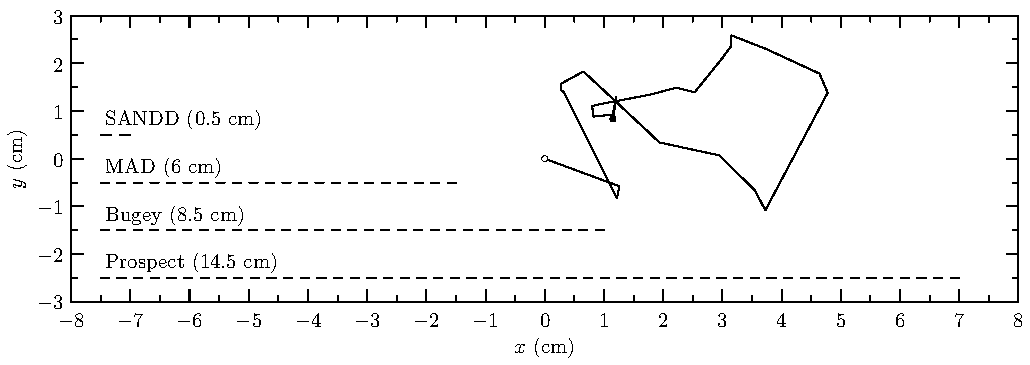
\includegraphics[width=17.405cm,height=7.653cm]{fig/asy_fig_1_paperB.pdf}
    \caption{Diagram showcasing relative scale for characteristic $n~xy$-trajectory projection from IBD vertex to capture location, as well as dimensions of segments in four 2D-segmented detectors: SANDD, MAD, Bugey, and PROSPECT. }
    \label{fig_segmentation_scaling}
\end{figure} % Top Left Block
  \end{rblock}

  \vspace{\rblockgap}

  \begin{rblock}{Traditional Approach}
    % ---- Top row: bullets + Chooz uncertainty plot, side by side ----
\begin{minipage}[t]{0.56\linewidth}
\begin{itemize}
    \item Conventional uncertainty calculation:
    \begin{equation}
      \boxed{\Delta \varphi = \arctan \left( \frac{P/l}{\sqrt N} \right)}
      \label{eq:deltaphi}
    \end{equation}
    \item If mean position resolution \(P\rightarrow0\), angular uncertainty \(\Delta\varphi\rightarrow0\) -- unphysical!
    \item Vogel and Beacom model shows a large spread (\(\sim26^\circ\)) in intial neutron direction
    \item Neutrons scatter many times before capture
\end{itemize}
\end{minipage}
\hfill
\begin{minipage}[t]{0.40\linewidth}
    \vspace{0pt}
    \centering
    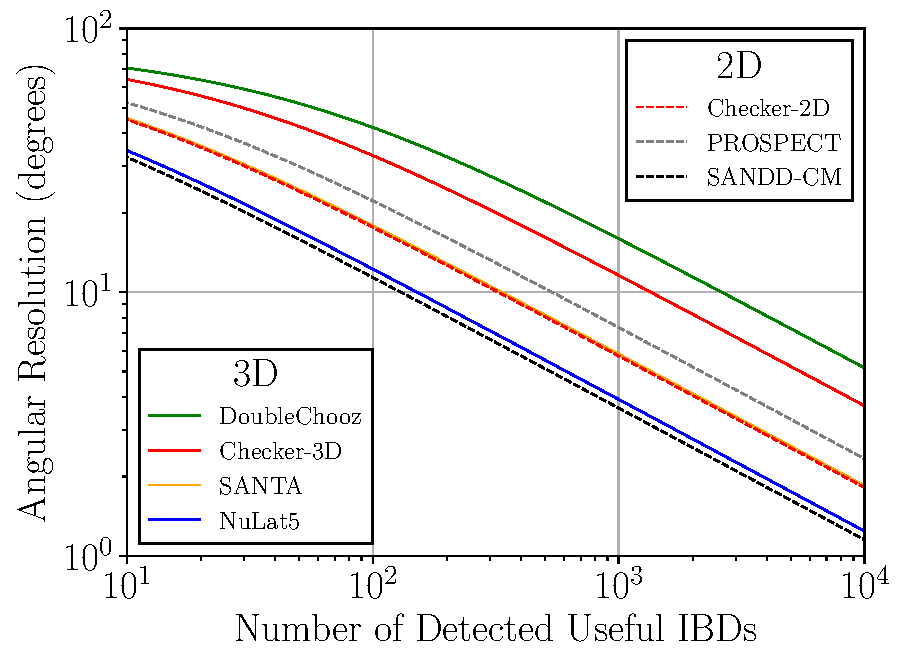
\includegraphics[width=\linewidth]{fig/angular_resolution_analytic_ylog_PackFactor_v2Useful.pdf}
    \captionof{figure}{Angular uncertainty calculated using the conventional ``Chooz'' approach, used in our previous study~[2].}
    \label{fig_old_method}
\end{minipage}

\vspace{0.5cm}

% ---- Additional content from Paper A: psi-geometry diagram, full width, scaled to fit ----
\begin{center}
\setlength{\unitlength}{.1\linewidth}
\resizebox{0.62\linewidth}{!}{%
\begin{picture}(10,4)
  \put(10,3){\color{gray}\line(-1,0){4}} % neutrino
  \put(10,3){\vector(-1,0){1.5}} % neutrino

  \put(1,3){\vector(1,0){1}} % x axis
  \put(1,3){\vector(0,1){1}} % y axis
  \put(1,3){\vector(-1,-2){.3}} % z axis
  \put(1.75, 2.65){$x$}
  \put(0.65, 3.65){$y$}
  \put(0.45, 2.45){$z$}

  \put(6,3){\color{black}\circle*{.25}} % IBD vertex
  \put(6.5,1.5){\color{black}\circle*{.25}} % e+ annihilation
  \put(1,.5){\color{black}\circle*{.25}} % n capture

  \put(6,3){\vector(-1,-0.2){1}} % neutron
  \put(6,3){\vector(.5,-1.5){.25}} % e+
  \put(6,3){\line(.5,-1.5){.5}} % e+
  % text:
  \put(5.7, 3.5){\text{IBD}}
  \put(5., 3.){\text{n}}
  \put(8.6, 3.5){$\bar\nu_e$}
  \put(6.4,2.4){\text{e}$^+$}
  \put(7.,1.3){\text{e}$^+$ \text{annihilation}}
  \put(0,0){\text{neutron capture}}

  % direction vectors:
  \put(1,.5){\vector(1,0){4}} % S_T
  \put(1,.5){\color{gray}\line(6.5,1.9){5.3}} % gray line along S_R
  \put(1,.5){\vector(6.5,1.9){3.5}} % S_R
  % text:
  \put(4.7,0){$S_T$}
  \put(3.7,1.8){$S_R$}

% THE MAIN ANGLE PSI:
  \put(2.7,0.7){\texttt{$\psi$}}
  \put(1,.5){\arc[0,16.5]{1.55}} % angle phi_nu
  \put(1,.5){\arc[0,16.5]{1.5}} % angle phi_nu
\end{picture}%
}
\end{center}
\captionof{figure}{Definition of the reconstruction angle $\psi$ between the true source direction $S_T$ and the reconstructed direction $S_R$ (neutron-capture vertex $\rightarrow$ positron-annihilation vertex). The antineutrino source lies along $x$; $\psi = 0$ is perfect reconstruction.}
\label{fig:recon}
% --- Original (full) caption, kept for reference / restore: ---
% Diagram of how the angle $\psi$ between reconstructed $S_R$ and true $S_T$ source direction is defined.
% The vector $S_R$ points from the reconstructed vertex of the neutron capture towards the reconstructed vertex where positron deposited its energy before annihilating. The MeV-scale positron travels a few millimeters before being annihilated with an electron.
% The keV-scale neutron loses its energy in the detector medium before being captured; the separation between IBD vertex and the capture location could be made large if there is no medium in between, as in some of the detector designs considered in this study.
% The antineutrino source was positioned along the $x$-axis: angle $\psi = 0$ would indicate a perfect reconstruction of direction.
 % Bottom Left Block
  \end{rblock}

\end{minipage}%
\hspace{\postermargin}%
\begin{minipage}[t][\bodyheight][t]{\colwidth}
  \begin{rblock}{Our Approach to Simulation Design}
    \begin{itemize}
    \item Used RATPAC-2 for all simulations
    \item Created simple monolithic geometry using \(0.1\%\)-wt \({}^6\text{Li}\)-doped plastic scintillator
    \item Created grid overlay to create binning matrices for 5 mm, 50 mm and 150 mm segment sizes in analysis work
\end{itemize}

\vfill

% The overpic call-out boxes extend above the image top edge, so keep
% clearance below the bullets; figure + caption share one centered
% minipage so the caption stays aligned with the image.
\vspace{0.5cm}
\begin{figure}
\centering
\begin{minipage}{0.62\linewidth}
    \centering
    \begin{overpic}[width=0.81\linewidth]{fig/RAT_PAC_IBD_run_6_5_crop.png}
      \footnotesize

    \put(16.5,90){\color{white}\vector(0,-1){5}}
    \put(0,93){\fcolorbox{white}{white!30}{\parbox{170pt}{neutron capture ${\color{orange}n} \; {^6}\mathrm{Li} \to {^3}\mathrm{H}\;\; {^4}\mathrm{He}$}}}

    \put(67,45){\color{white}\vector(0,1){15}}
    \put(57,41){\fcolorbox{white}{white!30}{\parbox{140pt}{positron\\ annihilation ${\color{red}e^+} e^- \to {\color{green}\gamma} \; {\color{green}\gamma}$}}}

    \put(81,86){\color{white}\vector(0,-1){15}}
    \put(65,85){\fcolorbox{white}{white!30}{\parbox{150pt}{inverse $\beta$ decay $\bar\nu_e \; ^1\mathrm{H} \to {\color{red}e^+ } \;{\color{orange}n}$}}}
    \end{overpic}
    \caption{RAT-PAC 2 rendering of an IBD event: positron track red, neutron --- orange, gamma-rays --- green, Cherenkov photons --- cyan (scintillation light off for clarity).}
    \label{fig_RATPAC_IBD_visual}
\end{minipage}
\end{figure}

\vfill
 % Top Center Block
  \end{rblock}

  \vspace{\rblockgap}

  \begin{rblock}{Novel Algorithm for Segmented Detectors}
    \begin{itemize}
    \item Generate reference data for all incident angles \\ This is done by rotating the grid overlay on simulation data and then performing the binning described below
    \item Bin prompt and delayed displacement vectors in matrix form by counting the number of voxels separating the IBD vertex and the capture vertex. Normalize all matrices for reference angles
    \item Create binning matrix for data set and normalize it
    \item Compute the \(L^2\) norm for the matrix differences for all reference angles
    \item Fit \(\alpha\left|\sin{\left(\frac{\theta-\theta_0}{2}\right)}\right|\) to \(L^2\) norms as a function of angle. The minimum gives the \(\theta_0\) fit parameter for the direction of the neutrino source.
\end{itemize}

\vspace{2cm}

\begin{figure}[ht]
        \setlength{\unitlength}{.04\linewidth}
        
    \begin{minipage}[t]{0.48\linewidth}
        \centering
\begin{picture}(10,5)
  \footnotesize
        \multiput(5,0)(.5,0){9}{\color{black}\line(0,1){4}} 
        \multiput(5,0)(0,0.5){9}{\color{black}\line(1,0){4}} 

        \multiput(5,4)(.5,0){9}{\color{black}\line(1,1){1}} 
        \multiput(9,0)(0,.5){9}{\color{black}\line(1,1){1}} 

        \put(10,1){\line(0,1){4}}
        \put(6,5){\line(1,0){4}}

        
          \thicklines
        \multiput(6.5, 2.50)(.025,0){20}{\color{black}\line(0,1){0.5}} 
        \multiput(0, 5)(.025,0){20}{\color{black}\line(0,-1){0.5}} 
        
        \multiput(6, 1.50)(.025,0){20}{\color{gray}\line(0,1){0.5}} 
        \multiput(0, 4.25)(.025,0){20}{\color{gray}\line(0,-1){0.5}} 
          \thinlines

        \put(0.8,4.7){prompt segment}
        \put(0.8,3.9){delayed segment}


        \put(1,1){\vector(-1,-1){1}} 
        \put(1,1){\vector(0,1){2}} 
        \put(1,1){\vector(1,0){2}} 

        \put(1,1){\vector(2,1){2}} 
        \put(1,1){\arc[0,26]{1}} 
        \put(1,1){\arc[0,26]{.95}} 

        
        \put(0,0.3){$z$}
        \put(0.7,2.8){$y$}
        \put(2.8,.7){$x$}
        \put(2.7,2){$\nu$}
        
       \put(6.75,-0.1){\color{black!90}\vector(0,1){4.7}} 
        \multiput(6.7,0.)(0,.25){16}{\color{blue}\line(1,0){0.1}}
        \put(4.8,2.75){\color{black!90}\vector(1,0){4.8}} 
        \multiput(5,2.7)(.25,0){16}{\color{blue}\line(0,1){0.1}} 

        \put(6.8,4.55){\color{black}$y'$}
        \put(9.2,2.4){\color{black}$x'$}
        \put(5.85,2.1){\color{black}$\theta_n^i$}


        \put(6.75,2.75){\color{blue}\arc[0,245]{0.65}} 
        \put(6.75,2.75){\color{blue}\vector(-1,-2){0.5}} 

        
        \multiput(3.5, 0.5)(0,1){4}{\color{black}\vector(2,1){1}} 
        
       \put(2,0){neutrino wind} 
        \put(2.2,1.2){$\vartheta_\nu$}
\end{picture}

    \end{minipage}
    \hfill
    \begin{minipage}[t]{0.48\linewidth}
        \centering

%        \setlength{\unitlength}{.1\linewidth}
\begin{picture}(10,4)
  \footnotesize

        \multiput(3,0.5)(.5,0){6}{\color{black}\line(0,1){2.5}} 
        \multiput(3,0.5)(0,0.5){6}{\color{black}\line(1,0){2.5}} 


        
          \thicklines
        \multiput(4., 1.50)(.025,0){20}{\color{black}\line(0,1){0.5}} % vertical
          \thinlines

 
        \put(4.25,0){\color{black}\vector(0,1){4}} 
        \put(2.5,1.75){\color{black}\vector(1,0){5}} 
        \multiput(4.2,0.25)(0,.5){7}{\color{blue}\line(1,0){0.1}}
        \multiput(2.75,1.7)(.5,0){7}{\color{blue}\line(0,1){0.1}} 

        \put(3.9,3.7){\color{black}$y$}
        \put(7.3,1.4){\color{black}$x$}


        \put(4.25,1.75){\color{blue}\arc[0,45]{2}} 
        \put(2.5,0){\color{blue}\vector(1,1){4}} 
        \put(5.7,3.7){\color{black}$45^\circ$}

        \put(2.5,0.5){\color{blue}\vector(7,5){5}} 
        \put(2.5,1){\color{blue}\vector(7,3){5}} 
        \put(2.5,1.5){\color{blue}\vector(7,1){5}} 

        \put(2.5,1.25){\color{red}\vector(7,2){5}} 
        \put(7.5,2.5){\color{red}$\theta_\nu^{exp}$}
         \put(7.5,2.){\color{blue}$\theta_\nu^{MC_1}$}
        \put(7.5,3){\color{blue}$\theta_\nu^{MC_2}$}
        \put(7.5,3.7){\color{blue}$\theta_\nu^{MC_3}$}
     

\end{picture}
\end{minipage}
        \caption{Diagram explaining the prompt-delayed segment geometry, as well as neutrino and axes orientation. 
%        In this work we assume that neutrino ``wind'' is in $xy$ plane, at an angle $\nu$ with the $x$ axis.
%        The prompt and delayed segment in this diagram shown for illustrative purposes; the actual separation depends on the segment size --- for large segments, prompt and delayed events would happen in the same segment. It is also illustrated that capture is not necessarily aligned with the neutrino beam (only on average it is the case as discussed in this paper).
%        To study the angular dependence we vary the angle of neutrino with respect to the detector's $x$ and $y$ axes (i.e. rotation of the detector along $z$ axis).}
}
        \label{fig:phi_def}
\end{figure}















% \begin{figure}[ht!]
%         \setlength{\unitlength}{.1\linewidth}
% \begin{picture}(10,4)

%         \multiput(3,0.5)(.5,0){6}{\color{black}\line(0,1){2.5}} 
%         \multiput(3,0.5)(0,0.5){6}{\color{black}\line(1,0){2.5}} 


        
%           \thicklines
%         \multiput(4., 1.50)(.025,0){20}{\color{black}\line(0,1){0.5}} % vertical
%           \thinlines

 
%         \put(4.25,0){\color{black}\vector(0,1){4}} 
%         \put(2.5,1.75){\color{black}\vector(1,0){5}} 
%         \multiput(4.2,0.25)(0,.5){7}{\color{blue}\line(1,0){0.1}}
%         \multiput(2.75,1.7)(.5,0){7}{\color{blue}\line(0,1){0.1}} 

%         \put(3.9,3.7){\color{black}$y$}
%         \put(7.3,1.4){\color{black}$x$}


%         \put(4.25,1.75){\color{blue}\arc[0,45]{2}} 
%         \put(2.5,0){\color{blue}\vector(1,1){4}} 
%         \put(5.7,3.7){\color{black}$45^\circ$}

%         \put(2.5,0.5){\color{blue}\vector(7,5){5}} 
%         \put(2.5,1){\color{blue}\vector(7,3){5}} 
%         \put(2.5,1.5){\color{blue}\vector(7,1){5}} 

%         \put(2.5,1.25){\color{red}\vector(7,2){5}} 
%         \put(7.5,2.5){\color{red}$\theta_\nu^{exp}$}
%          \put(7.5,2.){\color{blue}$\theta_\nu^{MC_1}$}
%         \put(7.5,3){\color{blue}$\theta_\nu^{MC_2}$}
%         \put(7.5,3.7){\color{blue}$\theta_\nu^{MC_3}$}
     

% \end{picture}
% \caption{A diagram explaining the idea behind a pattern-matching algorithm for IBD segmented detectors. The experimental/empirical data set (with {\it a priori} unknown neutrino angle $\theta_\nu^{exp}$) is compared against theoretical/simulation data sets (of known neutrino angles $\theta_\nu^{MC_i}$). Due to the symmetry and square geometry unique distributions only obtained between 0$^\circ$ and 45$^\circ$ angles. MC$_1$, MC$_2$, and MC$_3$ denote Monte Carlo data sets corresponding to that particular neutrino angle. The 5$\times$5 grid is shown for illustrative purposes.}
% \label{fig_algo_skewers}
% \end{figure} % Bottom Center Block
  \end{rblock}

\end{minipage}%
\hspace{\postermargin}%
\begin{minipage}[t][\bodyheight][t]{\colwidth}
  \begin{heroblock}{$\bigstar$\,Conclusions, Findings, and Future Work}
    \fbox
{
\begin{minipage}{0.45\textwidth}
    \vspace{0.5cm}
    Key findings:
    \begin{itemize}
        \item At large n, the algorithm gives the direction of antineutrino sources
        \item At small n, the algorithm gives a reasonable uncertainty
        \item As a pattern matching method, the algorithm provides a comparison between distributions
    \end{itemize}
\end{minipage}
}
\hspace{0.025\textwidth}
\begin{minipage}{0.45\linewidth}
\begin{figure}
    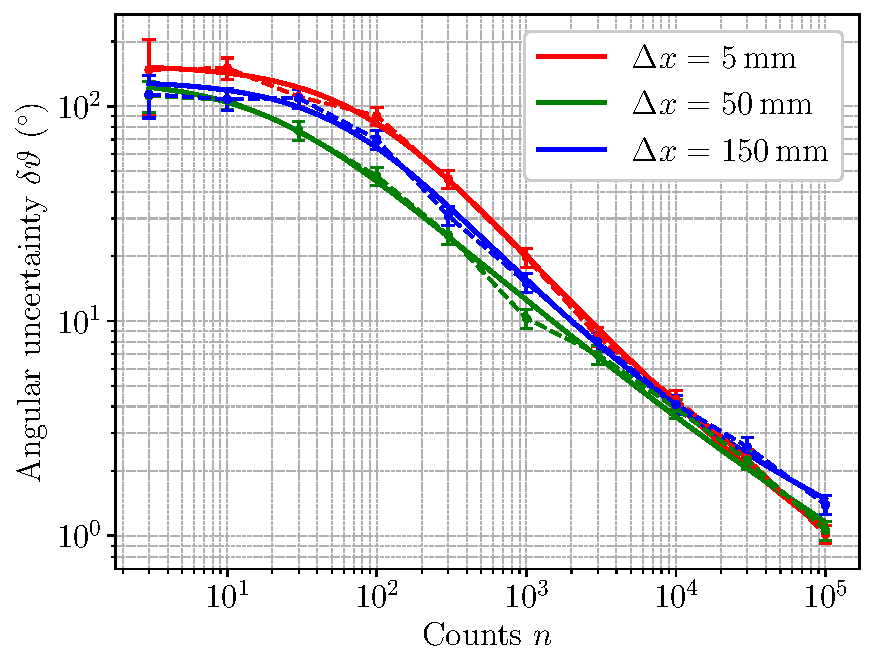
\includegraphics[width=0.7\linewidth]{fig/parallel/06_money_plot_fit_arctan_log_4p.pdf}

    \label{fig:POI_segsize_uncert}
\end{figure}
\end{minipage}
    \captionof{figure}{Angular uncertainty $\delta\vartheta$ versus event count $n$ for square segment sizes of 5, 50, and 150 mm.}
\vspace{0.5cm}

% ---- Figure 6: (a) binning distribution at theta=0  +  (b) sweet-spot plot ----
\begin{figure}
\centering
\begin{tabular}{cc}
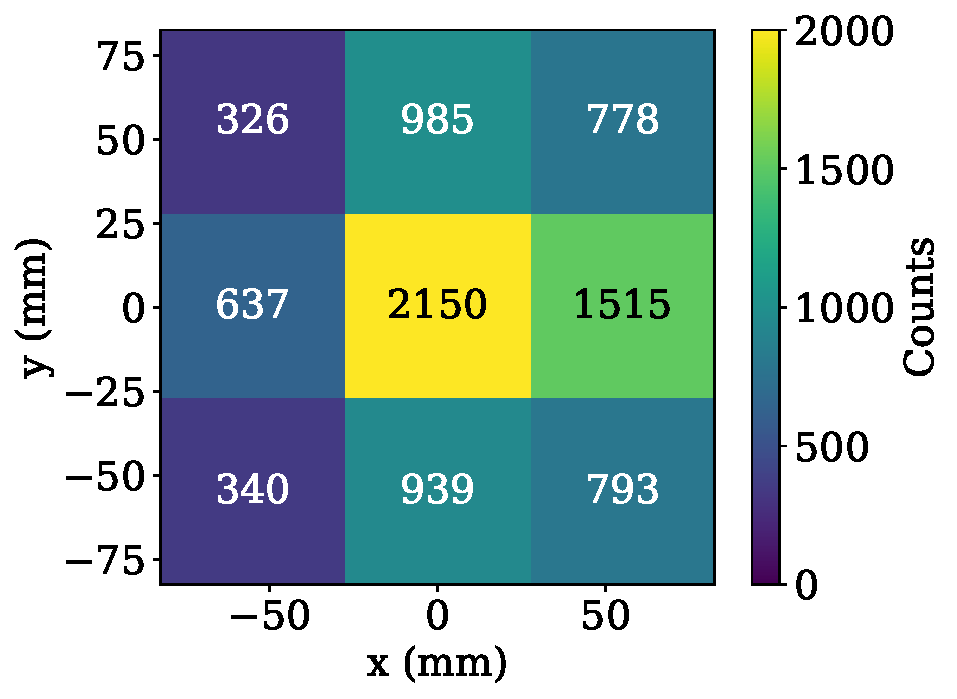
\includegraphics[width=0.32\linewidth]{fig/bin_dist_rot0_001wt.pdf}
&
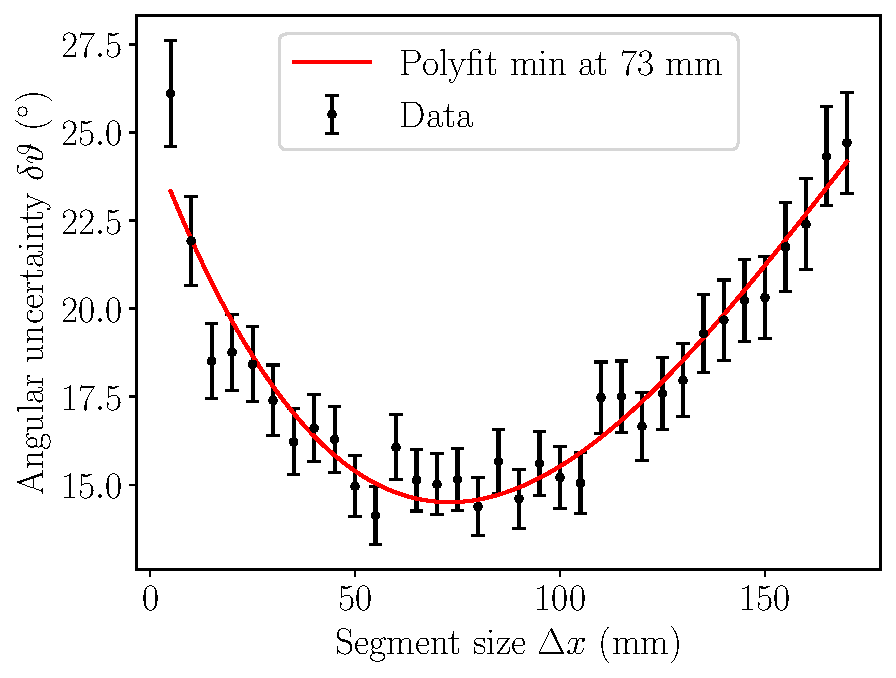
\includegraphics[width=0.45\linewidth]{fig/parallel/sweet_spot_final.pdf} \\
\end{tabular}

\begin{tabular}{>{\centering\arraybackslash}p{0.35\linewidth} >{\centering\arraybackslash}p{0.5\linewidth}}
    \makebox[0.35\linewidth][c]{%
        \begin{picture}(20,20)
            \put(-5,13){\color{black}\vector(1,0){20}}
        \end{picture}
    }
    &
    \\
    (a) binning distribution, $\vartheta_\nu = 0^\circ$ & (b) angular uncertainty vs.\ segment size
\end{tabular}
    \caption{(a) Binning distribution at $\vartheta_\nu=0^\circ$ (0.1\,wt\%\ ${}^6$Li; arrow marks the antineutrino direction); other incoming angles rotate the pattern. (b) Angular uncertainty versus segment size $\Delta x$, with a polynomial fit minimizing near $\Delta x\approx 73$ mm.}
    \label{fig:binning_sweetspot}
\end{figure}

\begin{center}
\highlight{Optimal segment size: $\Delta x \approx 73$ mm}
\end{center}
\vspace{0.3cm}

% ---- Figure 7: FND vs reference angle, labels on the plots (reference style) ----
\begin{figure}
\centering

\begin{minipage}{0.32\textwidth}
    \centering
    \begin{tikzpicture}
        \node[inner sep=0]
            {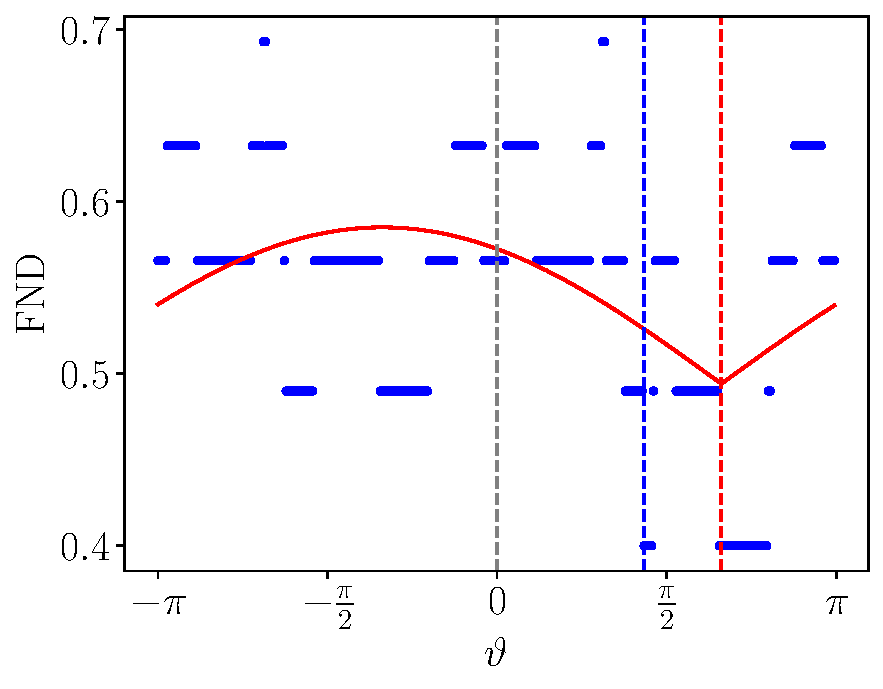
\includegraphics[height=1.675in]{fig/parallel/FND_n_10_dx_50.pdf}};

        \node[red, font=\fontsize{16}{19}\selectfont] at (1.85,2.225) {$\vartheta_\mathrm{fit}$};
        \node[blue, font=\fontsize{16}{19}\selectfont] at (1.15,2.225) {$\vartheta_\mathrm{min}$};
        \node[gray!50!black, font=\fontsize{16}{19}\selectfont] at (0.25,2.225) {$\vartheta_\mathrm{true}$};
    \end{tikzpicture}

    \vspace{2pt}
    (a) $n=10$
\end{minipage}
\hfill
\begin{minipage}{0.32\textwidth}
    \centering
    \begin{tikzpicture}
        \node[inner sep=0]
            {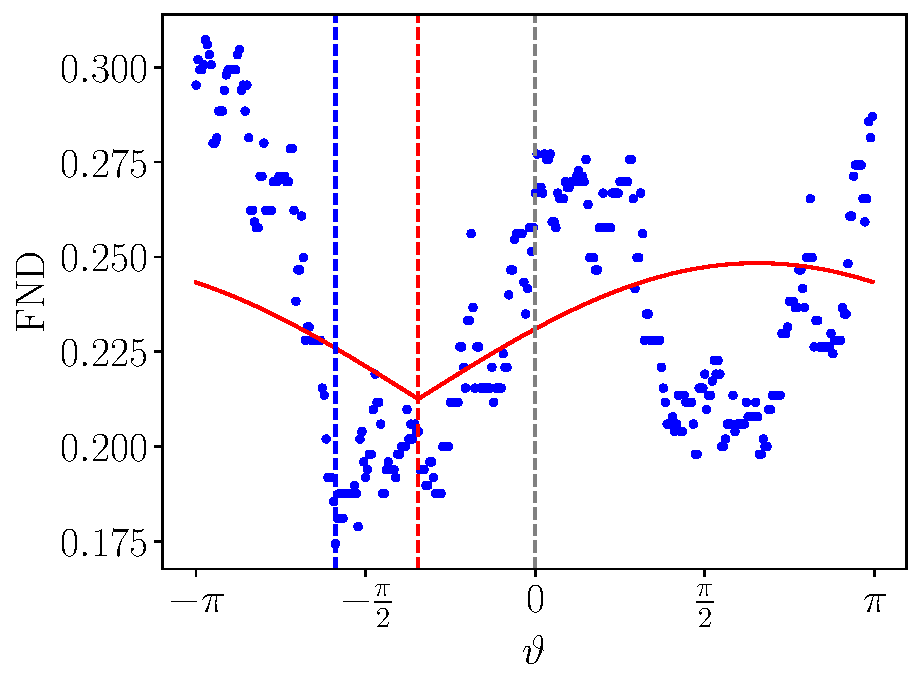
\includegraphics[height=1.675in]{fig/parallel/FND_n_100_dx_50.pdf}};

        \node[red, font=\fontsize{16}{19}\selectfont] at (-0.25,2.23) {$\vartheta_\mathrm{fit}$};
        \node[blue, font=\fontsize{16}{19}\selectfont] at (-0.9,2.23) {$\vartheta_\mathrm{min}$};
        \node[gray!50!black, font=\fontsize{16}{19}\selectfont] at (0.45,2.23) {$\vartheta_\mathrm{true}$};
    \end{tikzpicture}

    \vspace{2pt}
    (b) $n=100$
\end{minipage}
\hfill
\begin{minipage}{0.32\textwidth}
    \centering
    \begin{tikzpicture}
        \node[inner sep=0]
            {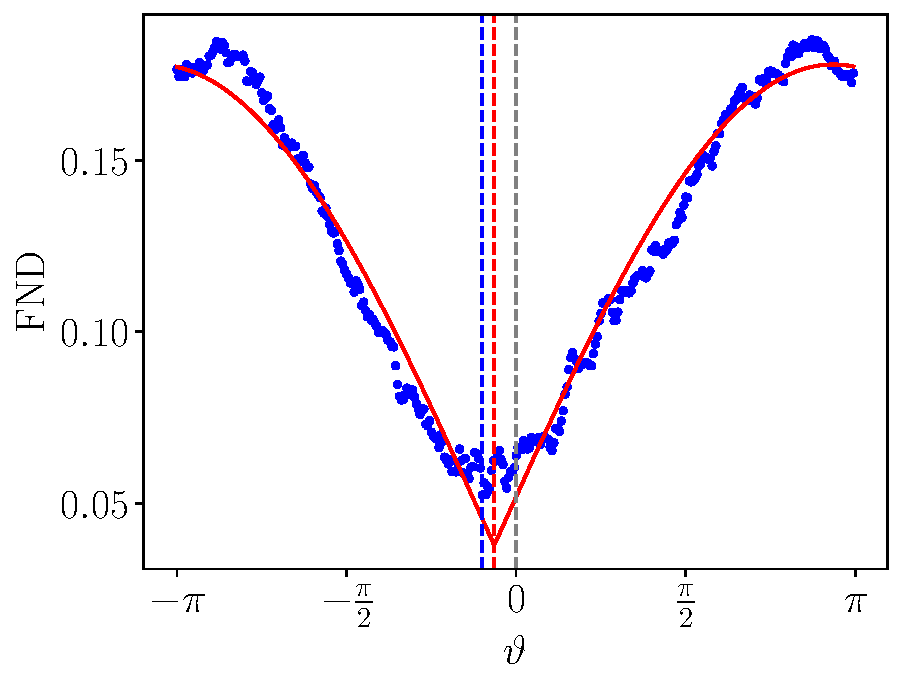
\includegraphics[height=1.675in]{fig/parallel/FND_n_1000_dx_50.pdf}};

        \node[red, font=\fontsize{16}{19}\selectfont] at (0.25,2.23) {$\vartheta_\mathrm{fit}$};
        \node[blue, font=\fontsize{16}{19}\selectfont] at (-0.4,2.23) {$\vartheta_\mathrm{min}$};
        \node[gray!50!black, font=\fontsize{16}{19}\selectfont] at (0.9,2.23) {$\vartheta_\mathrm{true}$};
    \end{tikzpicture}

    \vspace{2pt}
    (c) $n=1000$
\end{minipage}

\caption{FND versus reference angle $\vartheta$ at $n=10,100,1000$ (50 mm segments, RAT-PAC 2 capture data). As $n$ grows, the minimum $\vartheta_\mathrm{min}$ and arctan fit $\vartheta_\mathrm{fit}$ approach the true angle $\vartheta_\mathrm{true}$.}
\label{fig_spread}
\end{figure}


\fbox
{
\begin{minipage}{0.98\textwidth}
\vspace{0.5cm}
    Future work:
        \begin{itemize}
            \item Developing methods to take advantage of machine learning
            \item Investigating how to apply to monolithic detectors
            \item Investigating a generalized approach to three dimensionally segmented detectors
        \end{itemize}
\end{minipage}
}
 % Rightmost Block
    \vfill
  \end{heroblock}
\end{minipage}%
}% end centered body
%\hspace*{0.020\paperwidth}%

% =====================================================================
%  FOOTER STRIP
% =====================================================================
\begin{tikzpicture}[remember picture,overlay]
  \fill[UHGold]
    ([yshift=5cm]current page.south west)
    rectangle ([yshift=5.6cm]current page.south east);
  \fill[UHGreen]
    (current page.south west)
    rectangle ([yshift=5cm]current page.south east);
  \node[anchor=center, text=white] at ([yshift=3.8cm]current page.south) {
    \begin{minipage}{\dimexpr\paperwidth-0.05\paperwidth\relax}
      \small

\begin{minipage}[t]{0.50\linewidth}
  \textbf{References}\par
  %\vspace{0.3em}
  \begin{minipage}[t]{0.48\linewidth}
    [1] Crow \emph{et al.}, in prep.\,(2026)\par
    [2] Duvall \emph{et al.}, Phys.\ Rev.\ Applied \textbf{22}, 054030 (2024)\par
    [3] Yepez \emph{et al.}, AIP Adv.\ \textbf{16}, 025110 (2026)
  \end{minipage}\hspace*{-5.5cm}%\hfill
   \begin{minipage}[t]{0.48\linewidth}
    arXiv: https://doi.org/10.48550/arXiv.2603.03561\par
    arXiv: https://doi.org/10.48550/arXiv.2402.01636\par
    arXiv: https://doi.org/10.48550/arXiv.2506.17360
  %   [4] Andriamirado \emph{et al.}\,(PROSPECT), Phys.\ Rev.\ D \textbf{111}, 032014 (2025)\par
  %   [5] Vogel \& Beacom, Phys.\ Rev.\ D \textbf{60}, 053003 (1999).
   \end{minipage}
\end{minipage}\hfill
\begin{minipage}[t]{0.40\linewidth}
  \textbf{Acknowledgments}\par
  \footnotesize
  This work was funded in-part by the Consortium for Monitoring, Technology, and Verification under Department of Energy National Nuclear Security Administration award number DE-NA0003920.
  Prepared by LLNL under Contract DE-AC52-07NA27344. LLNL-POST-XXXXXX.
  \par
\end{minipage}\hfill
\begin{minipage}[t]{0.05\linewidth}
    \centering
    \vspace{1.00cm}
    \textbf{Ref. [1]:}
\end{minipage}
\begin{minipage}[c]{0.0125\linewidth}
  \centering
  \vspace{2.85cm}
  
\includegraphics[width=2.75\linewidth]{nu2026_poster/content/ArXiV_QR_code.png}
  %\placeholder{4}{4}{QR\\preprint} 
\end{minipage}

    \end{minipage}
  };
\end{tikzpicture}
\end{frame}
\end{document}